\subsection{Regulering - Morten}

Regulering af luftfugtighed og temperatur er implementeret på stort set samme måde, så begge vil blive beskrevet i dette afsnit. Selve design og implementering er en kombination af PSoC3 hardwareblokke og software, til at styre disse hardwareblokke. Funktionerne dette afsnit omhandler, er funktionerne beskrevet under "Humidity" og "Temperature" i figur \ref{fig:KlasseDiagram}.

\textbf{Design}

Funktionerne til at styre reguleringen af temperatur og luftfugtighed er 

\begin{itemize}
\item \texttt{regTemp(float)}/\texttt{regHum(float)} - Skal starte reguleringen af hhv. temperatur og luftfugtighed
\item \texttt{stopTemp()}/\texttt{stopHum()} - Skal afbryde reguleringen
\item \texttt{pauseTemp()}/\texttt{pauseHum()} - Skal afbryde regulering når den kaldes, og igangsættes reguleringen når den kaldes igen
\end{itemize}

Det ønskes, at reguleringen skal foregå automatisk efter at være igangsat. Dertil benyttes timere til at, med faste mellemrum, generere interrupts, og reguleringen vil da foregå i Interrupt service rutinen. Da reguleringen ikke er noget der er tidskritisk vil disse ISR have lav prioritet.

Temperatur og luftfugtighed har forskellige forudsætninger, og det giver anledning til følgende designbeslutninger:
\begin{itemize}
\item Varmeudveksling med omgivelserne vil gøre, at systemets temperatur konstant vil falde og systemet skal derfor have tilført en bestemt mængde energi hele tiden. Da varmelegemet styres ved hjælp af et PWM signal, skal ISR'en udføre en PID regulering og output af denne skal bestemme Duty Cycle af PWM signalet. 
\item Under forudsætningen af at systemet er godt isoleret, vil luftfugtigheden ikke falde. Så snart temperaturen er stabil, vil luftfugtigheden også være stabil. Da øgningen af luftfugtighed foregår via åbning og lukning af en magnetventil, skal ISR'en blot vurdere om luftfugtigheden er for lav, og åbne for ventilen hvis den er.
\end{itemize}
Ydermere bemærkes det at
\begin{itemize}
\item Da systemet ikke underbygger en mulighed for aktivt at sænke luftfugtigheden, er det vigtigt, at reguleringen ikke tilføjer for store mængder fugtighed.
\item Da luftfugtigheden er afhængig af temperaturen er det vigtigt, at PID reguleringen ikke laver oversving, da dette kan resultere i for høj luftfugtighed.
\end{itemize}
\clearpage
Begge reguleringer kræver information vedrørende hhv. systemets aktuelle temperatur og luftfugtigheden, og til dette anvendes de funktionerne beskrevet i afsnittet \ref{Sensor} om sensoren.

Ligeledes laves der i ISR'erne, er en underrutine, der skal holde øje med stabiliteten af systemet ved at

\begin{itemize}
\item Monitorere hvorvidt systemet når de krævede niveauer indenfor den tilladte tid
\item Monitorere om systemet er stabilt og holder de krævede niveauer indenfor de tilladte grænser
\item Meddele brugeren hvis de to forrige punkter ikke overholdes
\end{itemize}

som er påkrævede funktionaliteter iht. kravspecifikationen.


\textbf{Implementering}

Alle \texttt{reg},\texttt{pause} og \texttt{stop} funktioner er implementeret ved hjælp af de standardfunktioner, der er tilknyttet de hardwareblokke, der blev benyttet til de forskellige formål; hver regulering havde sin egen timer blok og tilhørende funktioner, og temperaturreguleringen havde ligeledes en PWM blok, til styring af varmelegemet samt cirkulations-ventilatoren. Cirkulationsventilatorens duty-cycle sættes til en fast værdi.

Som eksempel på implementering af funktionerne vises \texttt{pauseHum()}:

\begin{figure}[H]
\centering
\fbox{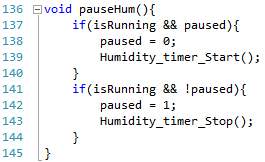
\includegraphics[scale=.80]{./7_projektbeskrivelse/design_og_implementering/software/billeder/pausehum.PNG}}
\caption[Diagram]{Implementering af \texttt{pauseHum()}}
\label{fig:PauseHum}
\end{figure}

Som det ses af Figur \ref{fig:PauseHum} benyttes funktionerne \texttt{Humidity\_timer\_Stop()} og \newline \texttt{Humidity\_timer\_Start()}, der starter og stopper for timeren, der skaber de interrupts, der foretager reguleringen af luftfugtigheden. De øvrige funktioner er implementeret på samme vis. Flagene \texttt{isRunning} og \texttt{paused} benyttes i rutinerne til at afgøre om ting startes, stoppes eller der ingenting skal foretages. Se kildekoden og dokumentation for flere detaljer ang. implementering af disse.

Selve reguleringen foregår ud fra differensen mellem de aktuelle og de ønskede værdier for temperatur og luftfugtighed; til regulering af luftfugtighed benyttes en simpel if-sætning, og til varmeregulering er implementeret følgende hjælpe-rutine:

\begin{figure}[H]
\centering
\fbox{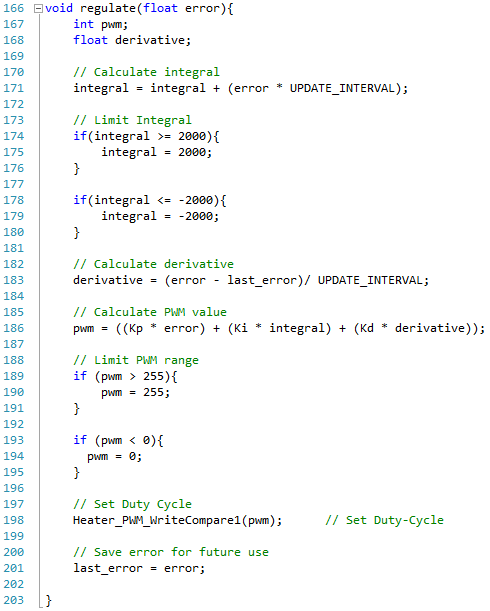
\includegraphics[scale=.80]{./7_projektbeskrivelse/design_og_implementering/software/billeder/pidroutine.PNG}}
\caption[Diagram]{PID hjælperutine}
\label{fig:PIDRutine}
\end{figure}

Som det ses af linie 198 anvendes igen standard funktioner.

Til at undersøge stabiliteten af systemet er implementeret en hjælpefunktion kaldet \texttt{stabilityControl(float)}. Den er opbygget af en kringlet mængde if-sætninger, flag og counters, så funktionaliteten kan bedst beskrives gennem dette flowchart:

\begin{figure}[H]
\centering
\fbox{\includegraphics[scale=0.8,page=5,trim=5mm 5mm 110mm 5mm]{./7_projektbeskrivelse/design_og_implementering/software/billeder/Varmeregulering.pdf}}
\caption[Diagram]{Flowdiagram for \texttt{stabilityControl(float)}}
\label{fig:stabilityControl}
\end{figure}

For mere information henvises til kildekoden.
